% !TEX root = ../main.tex

\section{Proposals}
\subsection{Proposal 1: Securing \textit{approve} method}
As discussed, a feasible solution would be to use CAS pattern to set new allowance atomically. This needs knowledge of transferred tokens that requires adding a new mapping variable to token code. The code would be still compatible with other smart contracts due to internal usage of the variable. Consequently, \textit{transferFrom} method will have an new line of code for tracking transferred tokens:
\begin{figure}[H]
	\centering
	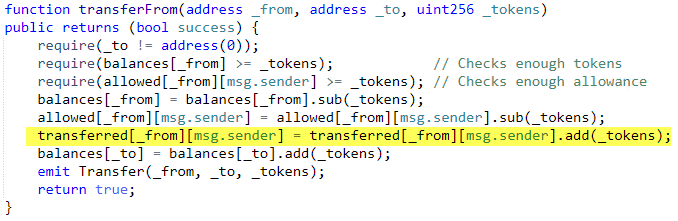
\includegraphics[width=1.0\linewidth]{figures/multiple_withdrawal_14.png}
	\caption{Modified version of \textit{transferFrom} based on added mapping variable.}
\end{figure}
\noindent Similarly, a block of code will be added to the \textit{approve} function to compare new allowance with transferred tokens. It has to work in both cases with zero and non-zero allowance set:
\begin{figure}[H]
	\centering
	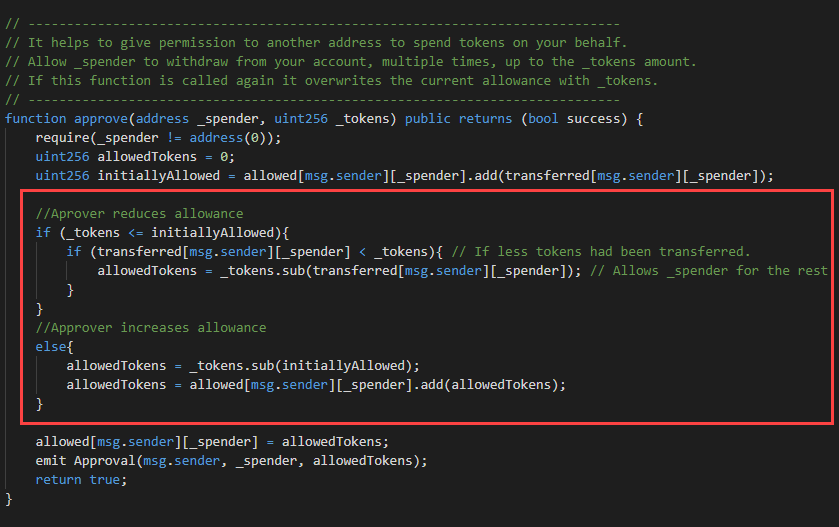
\includegraphics[width=1.0\linewidth]{figures/multiple_withdrawal_15.png}
	\caption{Added code block to \textit{approve} function to compare and set new allowance value.}
\end{figure}
\noindent Added code to \textit{approve} function will compare new allowance (\textit{\_tokens}) with current allowance of the spender (allowed[msg.sender][\_spender]) and with already transferred token (transferred[msg.sender][\_spender]). Then it decides to increase or decrease current allowance. If new allowance is less than initial allowance (sum of \textit{allowance} and \textit{transferred} variables), it denotes decreasing allowance, otherwise increasing allowance was intended. For example, we consider these scenarios:\newline\newline
\noindent \textbf{A.} Alice approves Bob for spending 100 tokens and then decides to decrease it to 10 tokens.
\begin{enumerate}
	\item Alice approves Bob for transferring 100 tokens.
	\item After a while, Alice decides to reduce Bob’s allowance from 100 to 10 tokens.
	\item Bob noticed Alice’s new transaction and transfers 100 tokens by front-running.
	\item Bob’s allowance is 0 and \textit{transferred} is 100 (set by \textit{transferFrom} function).
	\item Alice’s transaction is mined and checks initial allowance (100) with new allowance (10).
	\item As it is reducing, transferred tokens (100) will be compared with new allowance (10).
	\item Since Bob already transferred more tokens, his allowance will be set to 0.
	\item Bob is not able to move more than initial approved tokens.\newline
\end{enumerate}

\noindent \textbf{B.} Alice approves Bob for spending 100 tokens and then decides to increase it to 120 tokens.
\begin{enumerate}
	\item Alice approves Bob for transferring 100 tokens.
	\item After a while, Alice decides to increase Bob’s allowance from 100 to 120 tokens.
	\item Bob noticed Alice’s new transaction and transfers 100 tokens by front-running.
	\item Bob’s allowance is 0 and \textit{transferred} is 100.
	\item Alice’s transaction is mined and checks initial allowance (100) with new allowance (120).
	\item As it is increasing, new allowance (120) will be subtracted from transferred tokens (100).
	\item 20 tokens will be added to Bob’s allowance.
	\item Bob would be able to transfer more 20 tokens (120 in total as Alice wanted).
\end{enumerate}
In order to evaluate functionality of the new \textit{approve}/\textit{transferFrom} functions, we have implemented a standard ERC20 token (TKNv1\footnote{https://rinkeby.etherscan.io/address/0x8825bac68a3f6939c296a40fc8078d18c2f66ac7}) along side proposed ERC20 token (TKNv2\footnote{https://rinkeby.etherscan.io/address/0xf2b34125223ee54dff48f71567d4b2a4a0c9858b}). Result of tests for different input values shows that TKNv2 can address multiple withdrawal attack by making front-running gain ineffective. Moreover, we compared these two tokens in term of Gas consumption. TokenV2.\textit{approve} function uses almost the same amount of Gas as TokenV1.\textit{approve}, however, gas consumption of TokenV2.\textit{transferFrom} is around 50\% more than TokenV1.\textit{transferFrom}. This difference is because of maintaining a new mapping variable for tracking transferred tokens:
\begin{figure}[H]
	\centering
	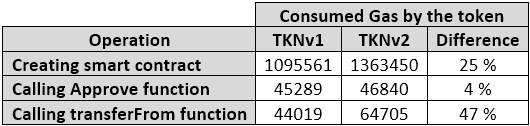
\includegraphics[width=1.0\linewidth]{figures/multiple_withdrawal_22.png}
	\caption{comparison of Gas consumption between TKNv1 and TKNv2.}
\end{figure}
\noindent In term of compatibly, working with standard wallets (like MetaMask) have not raised any transfer issue. This shows compatibility of the token with existing wallets.

\subsection{Proposal 2: Securing \textit{transferFrom} method}
Proposal 1 mitigates the attack in all situations, however it adjusts allowance based on transferred tokens. For example, if Alice allowed Bob for transferring 100 tokens and she decides to increase it to 120 tokens, the allowance will not directly set to 120 and the code adjusts it as below:
\begin{itemize}
	\item[-] If Bob already transferred 100 tokens, the new allowance will be 20 (100+20 = 120).
	\item[-] If Bob already transferred 70 tokens, the new allowance will be 50 (70+50 = 120).
	\item[-] If Bob has not already transferred any tokens, the new allowance will be 120 (0+120=120).\newline
\end{itemize}
\noindent Although the final result will be the same and does not allow Bob to transfer more than intended tokens, but ERC20 standard approve method emphasizes that:
\begin{figure}[H]
	\centering
	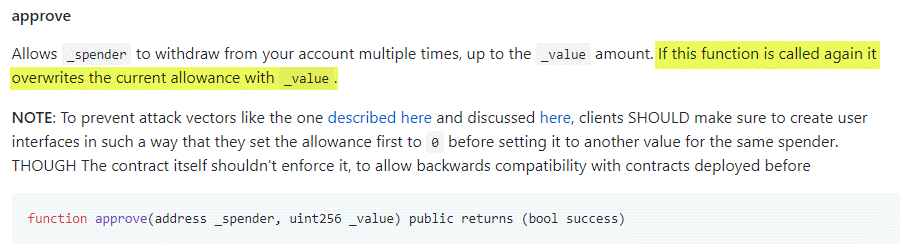
\includegraphics[width=1.0\linewidth]{figures/multiple_withdrawal_28.png}
	\caption{ERC20 \textit{approve} method constraint.}
\end{figure}
Hence, adjusting allowance will violate this constraint. On the other hand, this was the only solution for improving approve method. Because setting allowance securely to new values would need knowledge of transferred tokens. We can get this knowledge by:
\begin{enumerate}
	\item Tracking what have been transferred and ADJUST allowance accordingly.
	\item Passing a new input parameter that is showing what was the allowance before.
\end{enumerate}
We implemented the first approach and the second one would need to modify definition of \textit{approve} method. It seems that there is no feasible implementation to satisfy constraints of ERC20 and mitigating the attack under one solution. Therefore, we would assume API change as final solution of securing \textit{approve} method. As an alternative solution, we can think of securing \textit{transferFrom} method instead of \textit{approve} method. ERC20 standard emphasizes that:
\begin{figure}[H]
	\centering
	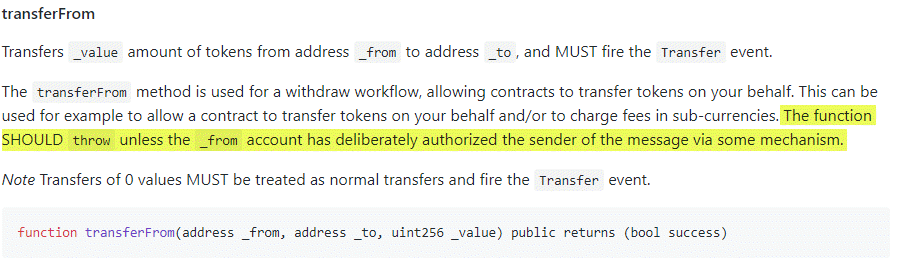
\includegraphics[width=1.0\linewidth]{figures/multiple_withdrawal_30.png}
	\caption{ERC20 \textit{transferFrom} method constraint.}
\end{figure}
So, the goal is to prevent spender from transferring more tokens than allowed by the approve. Based on this impression, we should not consider allowance as the main factor. Transferred tokens should be considered as the main variable in calculations. For example:
\begin{enumerate}
	\item Alice allowed Bob for transferring 100 tokens and decides to set it to 70 after a while.
	\item Bob front runs Alice’s transaction and transfers 100 tokes (legitimate transfer).
	\item Alice’s transaction is mined and sets Bob allowance to 80.
	\item Bob got new allowance and runs \textit{transferFrom(\_Bob,80)}. Since he already transferred more than 80, his transaction will fail and prevent multiple withdrawal.
	\item Bob’s allowance stays as 80, however, he can not use it.
\end{enumerate}
Here allowance can be considered as maximum allowance. It indicates that Bob is eligible to transfer up to specified limit if he has not already transferred any tokens. In fact, there is no relation between allowance (\textit{allowed[\_from][msg.sender]}) and transferred tokens (\textit{transferred[\_from][msg.sender]}). The fist variable shows maximum transferable tokens by a spender and can be changed irrelative to transferred tokens (approve method does not check transferred tokens). If Bob has not already transferred that much of tokens, he would be able to transfer difference of it \textit{allowed[\_from][msg.sender].sub(transferred[\_from][msg.sender]}). In other words, transferred is life time variable that accumulates transferred tokens regardless of allowance change. So, by this assumption, we can secure \textit{transferFrom} method instead of \textit{approve} method as below:
\begin{figure}[H]
	\centering
	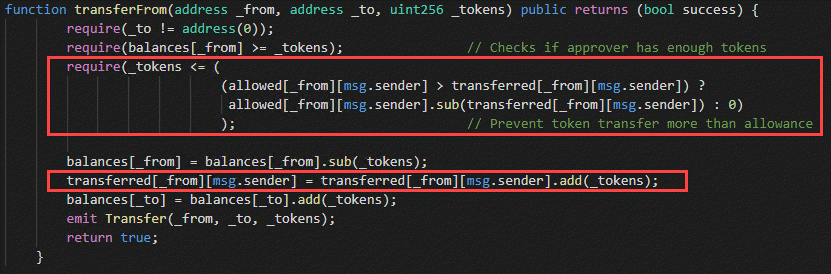
\includegraphics[width=1.0\linewidth]{figures/multiple_withdrawal_31.png}
	\caption{Securing \textit{transferFrom} method instead of \textit{approve} method.}
\end{figure}
\noindent This token is implemented as TKNv3 \footnote{https://rinkeby.etherscan.io/address/0x5d148c948c01e1a61e280c8b2ac39fd49ee6d9c6} on Rinkby network. Gas consumption of \textit{transferFrom} function is around 37\% more than standard implementation which is acceptable for having a secure ERC20 token.